\subsection{Czujnik światła i zbliżeniowy}
Testom poddano dane zebrane przez czujnik natężenia światła oraz czujnik zbliżeniowy.
Jeśli ktoś je przesłonił wartości zmieniały się jednocześnie.
Dodatkowo na odczyty czujnika natężenia miała wpływ pora dnia (rys. \ref{fig:DeviceLightRes}).
Dane zostały zebrane z okresu trzech dni.
\begin{figure}[htbp]
  \centering
  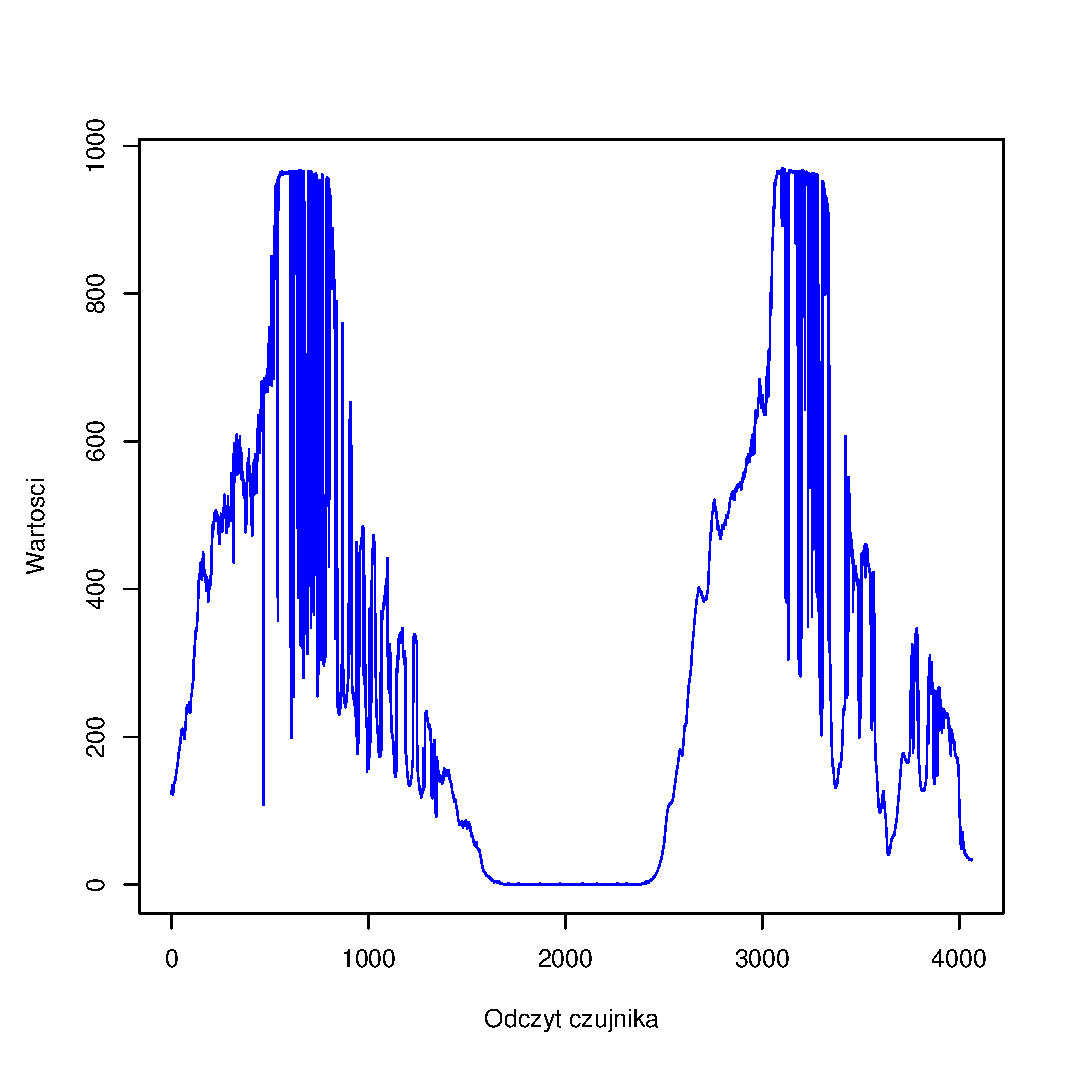
\includegraphics[width=0.6\textwidth]{img/ch-5-device-light}
  \caption{Odczyt czujnika światła -- dwa dni}
  \label{fig:DeviceLightRes}
\end{figure}

Zebrane dane analizowano jako dwa oddzielne strumienie jednowymiarowych próbek.
Jako poprawną zmianę przyjęto jednoczesne zasygnalizowanie zmian w obydwu badanych czujnikach.
Aby uznać zmianę za jednoczesną różnica czasowa pomiędzy próbkami może wynosić co najwyżej 20 próbek.

\subsubsection*{Czujnik światła}
Z uwagi na wrażliwość czujnika na porę dnia,
przekładającą się na wahania wartości algorytmy częściej powinny wykrywać zmiany.
Oczekiwania teoretyczne potwierdziły się -- tabela \ref{tab:LightResutl}.
Wszystkie algorytmy osiągneły zbliżony poziom, wykrywając zmianę średnio co 60 sekund.
\begin{table}[h]
  \label{tab:LightResutl}
  \centering
  \begin{tabular}{l r }
    Algorytm & \multicolumn{1}{l}{Liczba wykrytych zmian} \\
    \hline
    BAY & 4335  \\
    $\mbox{ADW}_{\mu}$ & 5050 \\
    $\mbox{ADW}_{d}$ & 4757  \\
  \end{tabular}
  \caption{Liczba wykrytych zmian -- czujnik światła}
\end{table}
\clearpage
\subsubsection*{Czujnik zbliżeniowy}
Charakterystyka tego czujnika jest bardziej stabilna.
Otrzymywane wartości ulegają zmianie, dopiero gdy coś się zbliża.
Widać to wyraźnie na otrzymanych wynikach (tabela \ref{tab:DistResutl}).
Liczba zaobserwowanych zmian jest mniejsza.
\begin{table}[h]
  \label{tab:DistResutl}
  \centering
  \begin{tabular}{l r }
    Algorytm & \multicolumn{1}{l}{Liczba wykrytych zmian} \\
    \hline
    BAY & 178 \\
    $\mbox{ADW}_{\mu}$ & 163 \\
    $\mbox{ADW}_{d}$ & 167\\
  \end{tabular}
  \caption{Liczba wykrytych zmian -- czujnik zbliżeniowy}
\end{table}

\subsubsection*{Wyniki sumaryczne}
Po skorelowaniu danych pojeńczych wyniki sumaryczne przedstawiono w tabeli \ref{tab:DevAllResutl}.
Niestety podobnie jak w przypadku testu skaczącej średniej algorytmy osiągnęły wysoki współczynnik fałszywych alarmów.
\begin{table}[h]
  \label{tab:DevAllResutl}
  \centering
  \begin{tabular}{l r}
    Algorytm & \multicolumn{1}{l}{Liczba wykrytych zmian} \\
    \hline
    BAY & 89 \\
    $\mbox{ADW}_{\mu}$ & 98 \\
    $\mbox{ADW}_{d}$ & 104 \\
  \end{tabular}
  \caption{Liczba wykrytych zmian -- wyniki sumaryczne}
\end{table}
Ponieważ analizowane dane pochodziły bezpośrednio z czujników,
nie były wcześniej przetwarzane,
to szum pomiarowy mógł mieć zauważalny wpływ na otrzymane wyniki.
Zastosowanie filtrów wygładzających przebiegi powinno obniżyć wskaźnik NPR.
